\section{Results}
\label{sec:results}

\begin{table}[t]
\centering
\caption{Macro-F1 ($\lambda=0$, mean of five seeds), classifier trained on Arabic script only. Bold: best deployable system per column; shaded: SelectNorm-adapt (primary). $^{\triangledown}$/$^{\blacktriangle}$: baseline significantly worse/better than SelectNorm-adapt (paired bootstrap, Holm-corrected $p<0.05$ over 20 comparisons per encoder; tested for B0, B1, B3, B4, SelectNorm-src). $^\dagger$Two passes; $^\ddagger$uses test labels.}
\label{tab:main}
\footnotesize\setlength{\tabcolsep}{3.2pt}
\begin{tabular}{@{}lrrrrrrrr@{}}\toprule
 & \multicolumn{4}{c}{\textbf{mE5}} & \multicolumn{4}{c}{\textbf{XLM-R}}\\
\cmidrule(lr){2-5}\cmidrule(lr){6-9}
 & $S_3$ & $S_4$ & $S_5$ & $S_6$ & $S_3$ & $S_4$ & $S_5$ & $S_6$\\\midrule
B0 original & 63.4$^{\triangledown}$ & 61.5$^{\triangledown}$ & 63.6$^{\triangledown}$ & \textbf{54.1} & 54.5$^{\triangledown}$ & 48.8$^{\triangledown}$ & 48.6$^{\triangledown}$ & 63.5$^{\triangledown}$\\
B1 always normalise & \textbf{82.0} & \textbf{67.2} & 69.4 & 52.9 & 72.8 & \textbf{64.5} & 63.1 & 72.3$^{\blacktriangle}$\\
B2 random, matched rate & 80.0 & 66.5 & 68.5 & 53.2 & 70.2 & 63.3 & 61.9 & 68.9\\
B3 confidence threshold & 82.0 & 67.2 & 69.4 & 52.9 & 72.9 & 64.4 & 63.0 & \textbf{72.3}$^{\blacktriangle}$\\
B4 direct gain & 81.4 & 67.0 & 69.9 & 53.6 & 73.5 & 63.9 & 63.3 & 68.7\\
B4b per-view loss & 81.6 & 67.1 & 69.9 & 53.7 & \textbf{73.9} & 63.9 & \textbf{63.4} & 68.2\\
SelectNorm-src & 81.3 & 67.0 & \textbf{70.0} & 53.7 & 73.8 & 63.8 & 63.4$^{\blacktriangle}$ & 68.0$^{\triangledown}$\\
\rowcolor{black!6}SelectNorm-adapt & 81.3 & 66.9 & 69.8 & 53.7 & 73.8 & 63.8 & 63.1 & 68.5\\
\quad Bayes threshold $\lambda\bar c$ & 81.4 & 66.9 & 69.6 & 53.5 & 73.9 & 64.0 & 63.4 & 69.0\\
\addlinespace[2pt]
R two-view ensemble$^\dagger$ & 78.9 & 66.5 & 69.7 & 54.4 & 67.3 & 57.2 & 54.7 & 69.7\\
B6 oracle$^\ddagger$ & 90.0 & 81.3 & 81.8 & 63.8 & 83.1 & 75.2 & 70.4 & 82.1\\
\midrule[\heavyrulewidth]
 & \multicolumn{4}{c}{\textbf{LaBSE}} & \multicolumn{4}{c}{\textbf{MARBERTv2}}\\
\cmidrule(lr){2-5}\cmidrule(lr){6-9}
 & $S_3$ & $S_4$ & $S_5$ & $S_6$ & $S_3$ & $S_4$ & $S_5$ & $S_6$\\\midrule
B0 original & 69.6$^{\triangledown}$ & 61.1$^{\triangledown}$ & 65.6$^{\triangledown}$ & \textbf{63.4}$^{\blacktriangle}$ & 64.3$^{\triangledown}$ & 62.4$^{\triangledown}$ & 60.0 & 52.5$^{\triangledown}$\\
B1 always normalise & 83.6 & \textbf{69.1} & 70.9 & 55.5$^{\triangledown}$ & 82.1 & 67.7 & 62.3 & 58.3\\
B2 random, matched rate & 81.0 & 67.3 & 69.5 & 60.4 & 79.9 & 67.3 & 61.9 & 56.7\\
B3 confidence threshold & 83.7 & 69.1 & 70.9 & 55.9$^{\triangledown}$ & \textbf{82.3} & 68.1 & 62.3 & \textbf{58.3}\\
B4 direct gain & 83.4 & 68.6 & 71.6 & 60.6 & 82.1 & 68.2 & \textbf{63.0} & 57.6\\
B4b per-view loss & 83.3 & 68.9 & \textbf{71.6} & 60.5 & 82.1 & 68.1 & 62.8 & 57.6\\
SelectNorm-src & 83.4 & 68.7 & 71.1 & 60.4$^{\triangledown}$ & 82.2 & 68.3 & 62.9 & 57.7\\
\rowcolor{black!6}SelectNorm-adapt & 83.4 & 68.8 & 71.5 & 60.9 & 82.1 & \textbf{68.3} & 62.9 & 57.7\\
\quad Bayes threshold $\lambda\bar c$ & \textbf{83.7} & 68.8 & 71.3 & 60.8 & 82.2 & 68.1 & 62.5 & 57.9\\
\addlinespace[2pt]
R two-view ensemble$^\dagger$ & 81.7 & 68.4 & 72.1 & 60.5 & 82.3 & 69.7 & 62.4 & 58.4\\
B6 oracle$^\ddagger$ & 91.5 & 82.2 & 85.7 & 75.2 & 93.6 & 84.2 & 77.6 & 70.4\\
\bottomrule\end{tabular}

\end{table}

\subsection{Selective normalisation against strong baselines (RQ1, RQ2)}
\label{sec:main-results}
Always normalising (B1) improves over the original input on the Tunisian and Algerian sets for every encoder, by 2.3--18.6 points (Table~\ref{tab:main}); on MYC it gains 8.8 points with XLM-R and loses 7.9 with LaBSE. Learned routing adds no consistent improvement. Against the direct-gain router B4 no difference is significant, and every 95\% interval lies inside $[-0.63,+0.58]$, within the 1-point margin in all 16 cells (a post hoc equivalence reading; Table~S1); SelectNorm-adapt and -src differ by $-0.25$ to $+0.54$ (three small differences significant). Against B1 and B3, SelectNorm-adapt is relevantly better in one cell (LaBSE, MYC: $+5.5$, $+5.0$), where normalising harms and thresholding fails to stop it, and relevantly worse in one (XLM-R, MYC: $-3.8$), where the router keeps the original view for about 40\% of inputs although normalising is right; in the LaBSE MYC cell it is also relevantly worse than B0, the better view there ($-2.5$). Elsewhere only 4 (B1) and 6 (B3) of 16 intervals lie within $\pm1$, and the other non-significant ones span $-1.3$ to $+2.4$, so small gains or losses cannot be excluded.

\subsection{Accuracy and cost (RQ3)}
\label{sec:cost}
\begin{figure}[t]
\centering
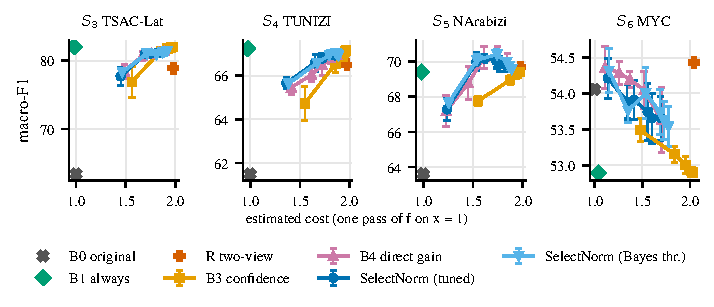
\includegraphics[width=\textwidth]{figures/pareto_lncs.pdf}
\Description{Four panels, one per test set, plotting macro-F1 against estimated inference cost for confidence thresholding, the direct-gain router and SelectNorm with tuned and Bayes thresholds, with single points for B0, B1 and the two-view ensemble.}
\caption{Macro-F1 against estimated cost (mE5, batch size 1, CPU; one pass of $f$ on $x$ = 1) for $\lambda\in\{0,.01,.02,.05,.1,.2\}$; bars: s.d.\ over seeds. Routers and B3 are charged the first pass and the normaliser (sunk) plus the second pass when selected; B1 the normaliser and one pass; R both passes.}
\label{fig:pareto}
\end{figure}
B0 costs 1.00 and B1 0.97--1.04 passes on $x$ (the normaliser adds about 0.4\%). At $\lambda=0$ SelectNorm-adapt costs 1.69--1.88 passes for mE5 and 1.43--1.88 across encoders, against 1.89--2.05 for the ensemble; raising $\lambda$ lowers the cost (mE5: 1.14--1.45 at $\lambda=0.2$) while macro-F1 falls towards B0 (Fig.~\ref{fig:pareto}). Routing is never cheaper than the better single view and never relevantly more accurate (at most $+0.6$, not significant); it saves compute only relative to running both views. End-to-end timing of the deployed pipeline (200 sentences per set; live decisions reproduce all 184{,}400 archived ones) agrees: B0 22--31\,ms; B1 0.91--1.05, SelectNorm-adapt 1.31--1.97, R 1.91--2.07 passes. Thresholding with each input's own cost $\lambda c_1(x)$ (exploratory) changes macro-F1 by $-2.0$ to $+0.6$ and cost by 0 to $-0.11$ passes, moving operating points along the same frontier (no worse on both in 29 of 80 cells, trading accuracy for cost in 48).

\subsection{Where per-input routing fails (RQ5)}
\label{sec:mechanism}
\begin{table}[t]
\centering
\caption{Mechanisms ($\Tcons$, Arabic-script $f$, five seeds). M1: disagreement rate (\%), AUC of target-cross-fitted $\hat\pi$. M2: win rate of $T(x)$ on disagreements (\%), AUC of source and of target-CV $\hat\rho$ (not deployable), calibration gap of source $\hat\rho$. M3: gain over the best view of $\hat\rho>\nicefrac12$. M4: oracle headroom, and the same minus the bootstrap-classifier reference. $^\circ$: AUC interval contains 0.5; $^{*}$: interval excludes 0 (95\%; Table~S4).}
\label{tab:mechanism}
\scriptsize\setlength{\tabcolsep}{2.6pt}
\begin{tabular}{@{}llrrrrrrrrrr@{}}\toprule
 & & \multicolumn{2}{c}{(M1) disagreement} & \multicolumn{4}{c}{(M2) direction} & \multicolumn{2}{c}{(M3) benefit} & \multicolumn{2}{c}{(M4) headroom}\\
\cmidrule(lr){3-4}\cmidrule(lr){5-8}\cmidrule(lr){9-10}\cmidrule(lr){11-12}
Enc. & Set & $P(D)$ & AUC$_\pi$ & $P(W|D)$ & AUC$_\rho$ & AUC$_\rho^{\rm tgt}$ & gap & $\Delta_{\rm src}$ & $\Delta_{\rm tgt}$ & oracle & vs.\ ref.\\\midrule
mE5 & $S_3$ & 34 & 0.68 & 77 & 0.66 & 0.64 & +3 & -0.6$^{*}$ & +0.0 & 8.0 & -0.3\\
 & $S_4$ & 33 & 0.64 & 57 & 0.56 & 0.58 & +19$^{*}$ & -0.3 & -0.1 & 14.1 & +4.6\\
 & $S_5$ & 29 & 0.62 & 58 & 0.63 & 0.57$^\circ$ & +15$^{*}$ & +0.2 & +0.7 & 12.4 & +3.2\\
 & $S_6$ & 21 & 0.74 & 47 & 0.54 & 0.56 & +20$^{*}$ & -0.5 & +0.2 & 9.7 & +4.6\\
\midrule
XLM-R & $S_3$ & 36 & 0.64 & 72 & 0.71 & 0.68 & +3 & +1.0$^{*}$ & +0.8 & 10.3 & +5.9\\
 & $S_4$ & 31 & 0.66 & 64 & 0.57 & 0.57 & +11$^{*}$ & -0.5 & +0.3 & 10.7 & +7.6\\
 & $S_5$ & 23 & 0.69 & 69 & 0.45$^\circ$ & 0.60$^\circ$ & +11$^{*}$ & +0.3 & -0.7 & 7.3 & +2.1\\
 & $S_6$ & 28 & 0.72 & 69 & 0.44 & 0.66 & -8$^{*}$ & -3.3$^{*}$ & +1.1$^{*}$ & 9.8 & +4.5\\
\midrule
LaBSE & $S_3$ & 30 & 0.69 & 73 & 0.61 & 0.53$^\circ$ & -0 & +0.1 & -0.1 & 7.9 & +1.3\\
 & $S_4$ & 34 & 0.65 & 62 & 0.57 & 0.59 & +6$^{*}$ & -0.4 & -0.4 & 13.0 & +5.7\\
 & $S_5$ & 34 & 0.65 & 58 & 0.59 & 0.55$^\circ$ & +3 & +0.4 & +0.2 & 14.9 & +7.5\\
 & $S_6$ & 31 & 0.68 & 33 & 0.57 & 0.64 & +16$^{*}$ & -2.6$^{*}$ & +0.8$^{*}$ & 11.8 & +5.3\\
\midrule
MARBERTv2 & $S_3$ & 39 & 0.69 & 70 & 0.63 & 0.60 & +1 & +0.1 & -0.3 & 11.5 & +0.8\\
 & $S_4$ & 37 & 0.71 & 60 & 0.61 & 0.64 & +13$^{*}$ & +0.4 & +2.8$^{*}$ & 16.5 & +2.0\\
 & $S_5$ & 31 & 0.73 & 57 & 0.63 & 0.54$^\circ$ & +13$^{*}$ & +0.2 & +1.1 & 15.3 & +3.6\\
 & $S_6$ & 30 & 0.71 & 59 & 0.55 & 0.63 & +4$^{*}$ & -0.3 & +1.1$^{*}$ & 12.1 & -0.7\\
\bottomrule\end{tabular}

\end{table}
\paragraph{(M1) Disagreement is moderately predictable.} 21--39\% of inputs change label under normalisation; the label-free estimate ranks them with AUC 0.62--0.74, all intervals within $[0.57,0.77]$ (Table~\ref{tab:mechanism}, Fig.~\ref{fig:diagmap}). Target re-estimation helps most on MYC (mE5: 0.67 to 0.74), but at $\lambda=0$ the rule depends on $\hat\rho$ alone.

\paragraph{(M2) Direction is weakly predictable from $z$, even in domain.} Source $\hat\rho$ reaches AUC 0.54--0.71 in 14 of 16 cells (upper bounds $\le0.76$); for XLM-R the interval includes 0.5 on Algerian text and lies below it on Moroccan text ($[0.41,0.48]$). Fitted on target labels by cross-validation, a reference no deployable system has, $\hat\rho$ reaches 0.53--0.68 (upper bounds $\le0.73$; five intervals include 0.5). With linear estimators the features carry little information about direction in any domain tested; better features or estimators are not excluded. What changes across domains is the \emph{level} of $\rho$: the win rate ranges from 33\% to 77\%, and source $\hat\rho$ is miscalibrated out of domain (gaps up to $+20$ points; intervals exclude zero in 11 of 12 cells).

\paragraph{(M3, M4) Benefit and headroom.} The rule $\hat\rho>\nicefrac12$ gains $-3.3$ to $+1.0$ points over the best view with source estimates (one interval above zero, three below) and $-0.7$ to $+2.8$ with the target-CV ceiling (upper bounds $\le+3.9$): most of the gap to the oracle remains when the router is fitted on the target. The oracle gains 7--17 points over the best view, but two classifiers differing only in a bootstrap resample of their training data show 3--15 points of such headroom on the same input; this reference depends on how the classifiers are made (2--6 with 80\% subsamples, 5--22 with weaker regularisation; Table~S5) and is not a decomposition.

\paragraph{Linguistic conditions.} On Tunisian and Algerian sets, always normalising helps less on inputs with many French or English tokens or low lexicon coverage, for every encoder except XLM-R on TUNIZI (French/English); negation and length show no consistent pattern. On MYC every condition changes sign with the encoder (Table~S6).

\subsection{Few target labels (RQ6), normaliser and classifier regime}
\label{sec:fewlabel}
With $k$ labelled target sentences, re-estimating the shift of $\hat\rho$ changes macro-F1 relative to zero-shot SelectNorm-adapt by $-1.4$ to $+1.5$ points across encoders, regimes, sets and $k$ (mean $-0.01$). Although targeted labels are $1/P(D{=}1)$ times more informative about the shift (Proposition~\ref{prop:efficiency}), targeted and random labels give results within $-0.1$ to $+0.2$ points of each other at every $k$ (averaged, descriptive). In the Arabic-script regime SelectNorm beats a set-level choice between B0 and B1 when $k\le16$ (by 2.6--2.9 points on average); the advantage shrinks to 0.3 points at $k=128$, consistent with M2.

\label{sec:normaliser}
The safeguards matter more than routing: always normalising with $T_{\rm lex}$ or $T_{\rm rule}$ loses 4--11 points on every set for mE5, and routing over them recovers only part of the loss (Table~S7). Keeping out-of-lexicon tokens in Latin script ($T_{\rm cov}$) reduces disagreements by about a third; it is worse than $\Tcons$ on the Tunisian sets and slightly better on $S_5$ and $S_6$. On NArabizi (RQ4), B1 agrees with $f$'s prediction on the human transliteration for 73--77\% of inputs, against 61--67\% for B0 and 73--76\% for SelectNorm-adapt; $f$ reaches 65--77 macro-F1 on the human transliterations. In the \textsc{+syn} regime (Table~S2) the original view improves, the win rate on disagreements moves towards 50\%, and SelectNorm-adapt is relevantly better than the better view once with Holm correction (MARBERTv2, $S_4$, $+1.1$) and twice more under the unadjusted criterion (mE5, $S_3$ $+2.1$, $S_4$ $+1.4$), and relevantly worse in two MYC cells under both (LaBSE $-2.4$, MARBERTv2 $-1.8$); it is never significantly better than B4 (worse once, $-0.4$).

\subsection{Qualitative examples}
\label{sec:qualitative}
% Qualitative examples. Values copied from results/qualitative/examples_mE5.json (archived per-example exports,
% re-checked against results/export/per_example and a rerun of T_cons). Provenance: docs/aciids2027/EXAMPLE_PROVENANCE.md
\begin{table}[t]
\centering
\caption{Test sentences with archived predictions (mE5, $\lambda=0$, SelectNorm-adapt): $x$ above $\Tcons(x)$; gold $y$ (1 = positive); posteriors $p_0$, $p_1$; routing $g$ and prediction $\hat y$ for seeds 0--4. Sources: TSAC test-file line (LGPL-3.0); NArabizi \texttt{sent\_id} (UD release, CC BY-SA 4.0); MYC row of \texttt{DATA\_CLEANED.csv}, text withheld (no licence).}
\label{tab:qualitative}
\footnotesize\setlength{\tabcolsep}{3pt}
\renewcommand{\arraystretch}{1.05}
\begin{tabular}{@{}l p{6.65cm} c c c l@{}}
\toprule
Source, effect & Original $x$ / normalised $\Tcons(x)$ & $y$ & $p_0$ & $p_1$ & seeds 0--4\\
\midrule
TSAC neg.\ 796 & \textit{mech 5arej 3lik el role} & 0 & .565 & .127 & $g$ \texttt{11111}\\
\quad help & \ar[0.8]{exAa} & & & & $\hat y$ \texttt{00000}\\
\addlinespace[1pt]
TSAC pos.\ 86 & \textit{Metrobi mouch kif ijale4 la5er} & 1 & .806 & .004 & $g$ \texttt{11111}\\
\quad harm & \ar[0.8]{exAb} & & & & $\hat y$ \texttt{00000}\\
\addlinespace[1pt]
NArabizi 2 & \textit{salem 3alikoum inchalah le pondium et les midailes d'or} & 1 & .175 & .842 & $g$ \texttt{11111}\\
\quad help & \ar[0.8]{exBa} & & & & $\hat y$ \texttt{11111}\\
\addlinespace[1pt]
NArabizi 4609 & \textit{oui le Maroc aktar jahiziya li had tasfiyat la 3ala lmostawa tandimi} & 1 & .519 & .088 & $g$ \texttt{11111}\\
\quad harm & \ar[0.8]{exBb} & & & & $\hat y$ \texttt{00000}\\
\addlinespace[1pt]
MYC 9079 & [withheld] two \textit{ma\ldots ch} negations split as \ar[0.8]{ma}\,\ldots\,\ar[0.8]{shin}, & 1 & .645 & .250 & $g$ \texttt{00111}\\
\quad harm (s2--4) & letter elongations squeezed, emoji kept & & & & $\hat y$ \texttt{11000}\\
\addlinespace[1pt]
MYC 14543 & [withheld] two Latin-script loanwords protected, & 1 & .480 & .302 & $g$ \texttt{00001}\\
\quad both wrong & negated verb split, emoji kept & & & & $\hat y$ \texttt{00000}\\
\bottomrule
\end{tabular}
\end{table}

Table~\ref{tab:qualitative} shows six hand-picked (not representative) test sentences. In TSAC~neg.~796 the negator \textit{mech} is mapped by the fixed list and French \textit{role} is protected; in TSAC~pos.~86, \textit{ijale4} and \textit{la5er} fall back to character rules. In both NArabizi sentences the French article \textit{le} is read as Arabizi (the context is mostly Arabizi) and mapped by the negator list to \ar{la} (\textit{no}), yet the normalised view is right in sentence~2 and wrong in 4609. The router selects the normalised view for all four in every seed: its features do not separate these cases. In MYC~9079 the decision varies with the policy split.
